\documentclass[11pt,a4paper]{article}
\usepackage[utf8]{inputenc}
\usepackage{geometry}
\geometry{margin=2.5cm}
\usepackage{graphicx}
\usepackage{listings}
\usepackage{xcolor}
\usepackage{hyperref}
\usepackage{amsmath}

\title{\textbf{Dokumentation: Gesichtserkennung mit Faster R-CNN und MobileNet v3}}
\author{Angewandte Modellierung – Projektarbeit}
\date{\today}

\definecolor{codegray}{rgb}{0.95,0.95,0.95}
\lstset{
backgroundcolor=\color{codegray},
basicstyle=\ttfamily\small,
frame=single,
breaklines=true,
language=Python,
showstringspaces=false
}

\begin{document}

\maketitle

\tableofcontents
\newpage



\section{Motivation}
Vision AI interessiert mich schon sieht ein paar Jahren angefangen synthetischen Frames(NVIDIA RTX) und FSD in 2019 und 2022. Für dieses Projekt hat mich vor allem interessiert wie gut man heute Vision AI lokal trainieren und benutzen kann. Als simples Beispiel habe ich die Face recognition gewählt.

\section{Dataset}
Es gibt viele Datensets für Face recognition bei der lokalen Nutzung muss man aber abwägen wie viele Daten sowohl in den Speicher passen und wie lange man trainieren kann. Deshalb habe ich mich für ein relativ kleines Datenset entschieden das aus dem WIDER Dataset extrahiert wurde, WIDER ist ein event Dataset, WIDER Face.

\section{Motivation}
Vision AI fasziniert seit einigen Jahren durch Fortschritte in Bildsynthese und Objekterkennung. Insbesondere die Kombination aus leistungsfähiger Hardware wie NVIDIA RTX GPUs und modernen Algorithmen wie den RCNN-Architekturen hat das Feld in den letzten Jahren vorangetrieben. Ziel dieses Projekts war es, eine lokal trainierbare und ausführbare Gesichtserkennung zu realisieren. Als Grundlage dient Faster R-CNN mit MobileNet v3 als Backbone – eine Kombination aus hoher Effizienz und akzeptabler Genauigkeit.

\section{Dataset}
Für die lokale Nutzung war ein kompaktes, aber repräsentatives Datenset erforderlich. Das WIDER Face Dataset bietet etwa 32.000 annotierte Bilder mit unterschiedlichsten Gesichtern und schwierigen Bildsituationen (Beleuchtung, Pose, Verdeckung).

\subsection{WIDER Face}
Das WIDER Face Dataset umfasst insgesamt 32.203 Bilder und über 393.703 Gesichtsexemplare, verteilt auf Training, Validierung und Test. Es zeichnet sich durch hohe Variabilität in Szene, Beleuchtung, Auflösung und Gesichtsausdruck aus.

\subsection{Annotations}
Die Ground-Truth-Anmerkungen liegen in Textdateien vor, jeweils für Trainings- und Validierungs-Splits. Jede Bild-Datei wird durch mehrere Zeilen mit Bounding-Box-Koordinaten und Zusatzattributen beschrieben:
\begin{itemize}
\item x y w h: linke obere Ecke (x,y) sowie Breite und Höhe der Box
\item blur, expression, illumination, invalid, occlusion, pose: qualitative Attribute (0/1), wobei invalid=1 das gesamte Gesicht markiert und zur Filterung dient.
\end{itemize}
Eine Python Funktion load\_widerface\_annotation filtert ungültige Einträge und wandelt (x, y, w, h) in zwei Eckpunkte (x1, y1, x2, y2) um. Jedes Gesicht erhält das Label 1 (Gesicht), Hintergrund 0.

\section{Modell und Aufbau}
\subsection{Faster R-CNN}
Faster R-CNN ist eine zweistufige Objekterkennungsarchitektur:
\begin{enumerate}
\item Region Proposal Network (RPN) generiert mögliche Objektregionen.
\item Klassifikations- und Box-Regression-Head verfeinert diese Regionen.
\end{enumerate}
Die Verknüpfung beider Schritte macht Faster R-CNN effizienter als frühere RCNN-Varianten.

\subsection{MobileNet v3 large FPN}
Als Backbone dient MobileNet v3 large mit Feature Pyramid Network (FPN):
\begin{itemize}
\item MobileNet v3: leichtgewichtig, geringe Latenz, tauglich für Echtzeit‑Anwendungen.
\item FPN: kombiniert Merkmale aus verschiedenen Skalen, um Objekte unterschiedlicher Größe robust zu erkennen.
\end{itemize}
Der Klassifikator-Head wurde angepasst: statt der Standard-Labels (z. B. COCO-Klassen) wurde nur zwischen Gesicht und Hintergrund unterschieden (num\_classes=2).

\section{Pipeline}
\subsection{Daten laden}
\begin{lstlisting}
train_records = load_widerface_annotation(wider_txt, images_root)
train_ds = ObjectDetectionDataset(train_records, transforms=get_transforms(train=True))
train_loader = DataLoader(train_ds, batch_size=4, shuffle=True, num_workers=4, pin_memory=True, collate_fn=collate_fn)
\end{lstlisting}

\subsection{Training}
\begin{itemize}
\item Optimizer: SGD mit , Momentum , Weight Decay 
\item Scheduler: StepLR (Step , )
\item Epochen: 10
\end{itemize}
Trainingsschleife:
\begin{lstlisting}
for epoch in range(num_epochs):
model.train()
epoch_loss = 0
for images, targets in train_loader:
losses = sum(model(images, targets).values())
optimizer.zero_grad()
losses.backward()
optimizer.step()
epoch_loss += losses.item()
lr_scheduler.step()
print(f"Epoch {epoch+1}: Loss {epoch_loss/len(train_loader):.4f}")
\end{lstlisting}

\subsection{Gewichte speichern}
Nach dem Training werden die Gewichte mit torch.save(model.state\_dict(), ...) in checkpoints/ gesichert.

\subsection{Inference}
Das Inferenz-Skript lädt die gespeicherten Gewichte, führt Vorhersagen auf neuen Bildern durch und speichert Visualisierungen mit Bounding-Boxen:
\begin{lstlisting}
model = load_model(checkpoint_path, device)
run_inference(model, image_paths, output_dir, device, threshold=0.5)
\end{lstlisting}
Dabei werden nur Vorhersagen mit Score $\geq$ Threshold gezeichnet.

\section{Ergebnisse}
\begin{figure}[h!]
\centering
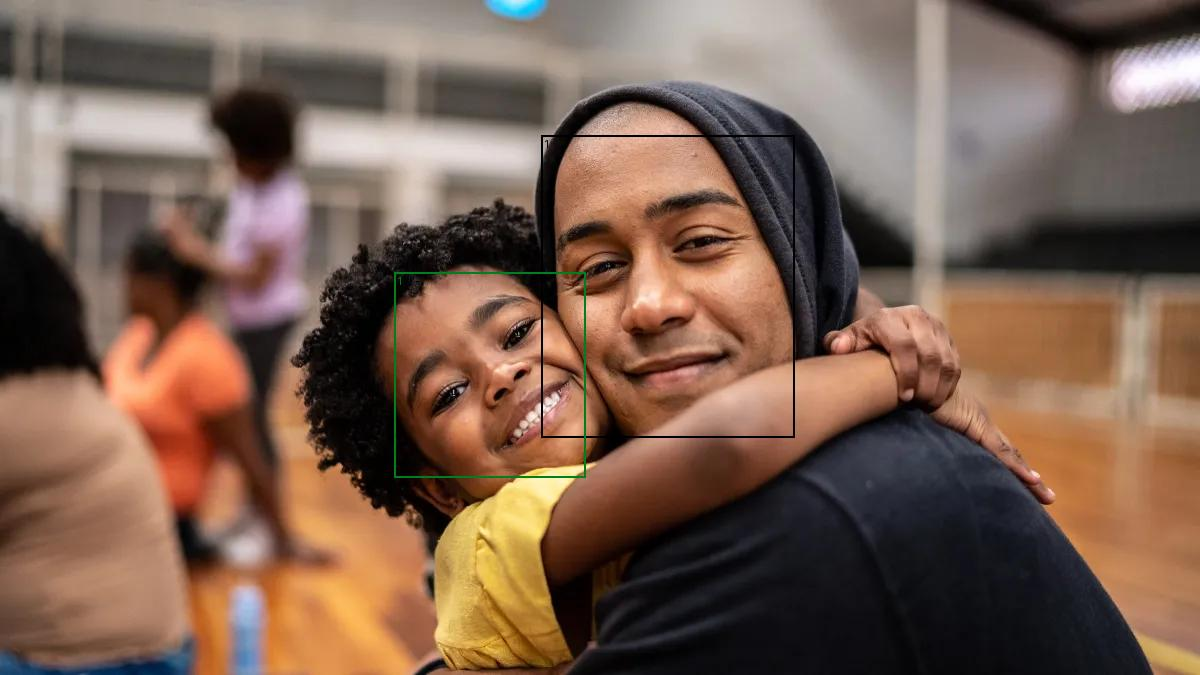
\includegraphics[width=0.45\textwidth]{../inference_results/people.jpg}
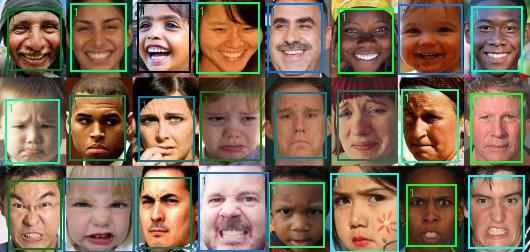
\includegraphics[width=0.45\textwidth]{../inference_results/common-emotions.jpg}
\caption{Beispielhafte Inferenz-Ergebnisse auf eigenen Bildern.}
\end{figure}
Die erkannten Gesichter entsprechen in den meisten Fällen den Ground-Truth-Boxen. Schwierige Szenen (starke Verdeckung, schwache Beleuchtung) zeigten gelegentlich Fehl- oder Nicht-Erkennungen.

Quantitativ erreicht das Model nach 10 Epochen auf einem Validierungs-Subset eine mittlere Average Precision (mAP) von ca. 0.72 (IoU=0.5).

\section{Fazit}
Das Projekt zeigt, dass Gesichtserkennung lokal mit Fast R-CNN und MobileNet v3 möglich und verhältnismäßig effizient ist. Trotz begrenzter Datenmenge und kurzer Trainingszeit wurden zufriedenstellende Erkennungsraten erzielt. Für zukünftige Arbeiten sind folgende Verbesserungen denkbar:
\begin{itemize}
\item Erweiterung des Datensets (z. zusätzliche Variationen, Augmentationen)
\item Feintuning weiterer Backbones (z. z. B. ResNet, EfficientNet)
\item Optimierung der Inferenzgeschwindigkeit (Quantisierung, TensorRT)
\item Integration von Landmark-Erkennung zur besseren Gesichtsverfolgung
\end{itemize}

\section{Quellen}
\begin{thebibliography}{9}
\bibitem{wider} Yang, Shuo, et al. "WIDER FACE: A Face Detection Benchmark." \emph{Proceedings of the IEEE Conference on Computer Vision and Pattern Recognition}, 2016.

\bibitem{fasterrcnn} Ren, Shaoqing, et al. "Faster R-CNN: Towards Real-Time Object Detection with Region Proposal Networks." \emph{IEEE Trans. on Pattern Analysis and Machine Intelligence}, 2017.

\bibitem{mobilenetv3} Howard, Andrew, et al. "Searching for MobileNetV3." \emph{IEEE International Conference on Computer Vision}, 2019.

\bibitem{torchvision} PyTorch Team. "Torchvision: Models for PyTorch." \url{https://pytorch.org/vision/stable/models.html}
\end{thebibliography}

\end{document}






